\section{VLSI layout}

The problem involves embedding a complete binary tree with $n$ leaves into a grid while minimizing the area used.
\begin{figure}[H]
    \centering
    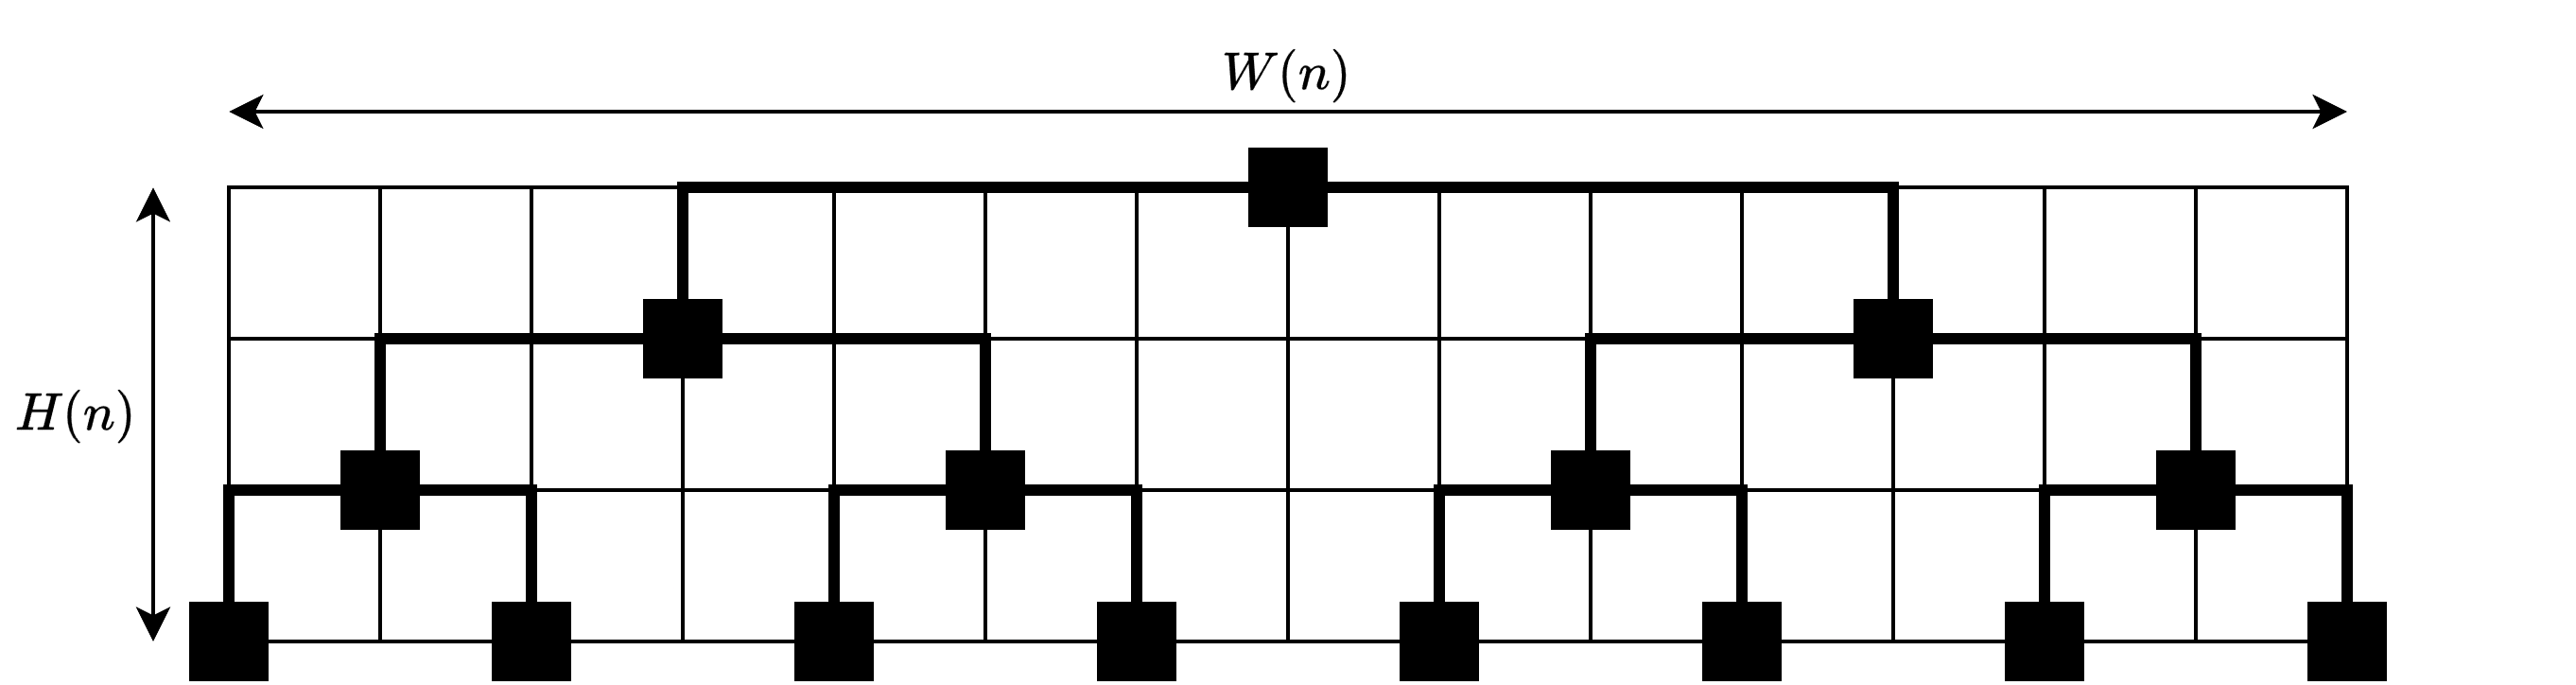
\includegraphics[width=0.9\linewidth]{images/vlsi.png}
    \caption{VLSI layout problem}
\end{figure}
For a complete binary tree, the height is given by:
\[H(n)=H\left(\dfrac{n}{2}\right)+\Theta(1)=\Theta(\log_2n)\]
The width is expressed as:
\[W(n)=2W\left(\dfrac{n}{2}\right)+\Theta(1)=\Theta(n)\]
Thus, the total area of the grid required is:
\[\text{Area}=H(n)\cdot W(n)=\Theta(n\log_2n)\]

An alternative solution to this problem is to use an $h$-tree instead of a binary tree.
\begin{figure}[H]
    \centering
    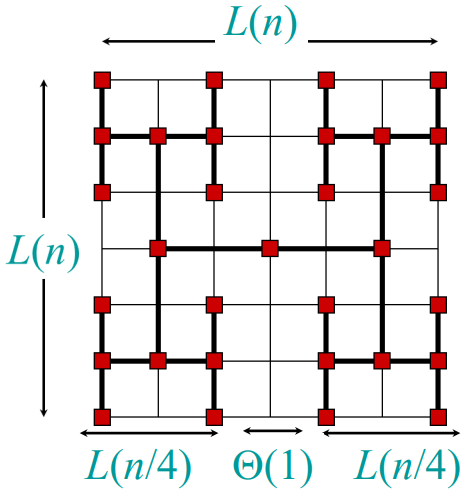
\includegraphics[width=0.65\linewidth]{images/vlsi1.png}
    \caption{VLSI layout problem}
\end{figure}
For the $h$-tree, the length is given by:
\[L(n)=2L\left(\dfrac{n}{4}\right)+\Theta(1)=\Theta(\sqrt{n})\]
Consequently, the total area required for the $h$-tree is computed as:
\[\text{Area}=L(n)^2=\Theta(n)\]